\documentclass[a4paper,10pt]{article}
\usepackage[utf8]{inputenc}
\usepackage[T1]{fontenc}
\usepackage{lmodern}
\usepackage[ngerman]{babel}
\usepackage{amsmath}
\usepackage{fullpage}
\usepackage{listings}
\usepackage{amssymb}
\usepackage{newclude}
\usepackage{multirow}
\usepackage{longtable}
\usepackage{graphicx}
%\pagestyle{empty}


\lstset{ %
  %backgroundcolor=\color{white},   % choose the background color; you must add \usepackage{color} or \usepackage{xcolor}
  %basicstyle=\footnotesize,        % the size of the fonts that are used for the code
  %breakatwhitespace=false,         % sets if automatic breaks should only happen at whitespace
  breaklines=true,                 % sets automatic line breaking
  %captionpos=b,                    % sets the caption-position to bottom
  commentstyle=\bf,    % comment style
  %deletekeywords={...},            % if you want to delete keywords from the given language
  %escapeinside={\%*}{*)},          % if you want to add LaTeX within your code
  %extendedchars=true,              % lets you use non-ASCII characters; for 8-bits encodings only, does not work with UTF-8
  frame=single,                    % adds a frame around the code
  %keepspaces=true,                 % keeps spaces in text, useful for keeping indentation of code (possibly needs columns=flexible)
  %keywordstyle=\color{blue},       % keyword style
  language=Java,                 % the language of the code
  %otherkeywords={*,...},            % if you want to add more keywords to the set
  numbers=left,                    % where to put the line-numbers; possible values are (none, left, right)
  %numbersep=5pt,                   % how far the line-numbers are from the code
  %numberstyle=\tiny\color{mygray}, % the style that is used for the line-numbers
  %rulecolor=\color{black},         % if not set, the frame-color may be changed on line-breaks within not-black text (e.g. comments (green here))
  %showspaces=false,                % show spaces everywhere adding particular underscores; it overrides 'showstringspaces'
  %showstringspaces=false,          % underline spaces within strings only
  %showtabs=false,                  % show tabs within strings adding particular underscores
  %stepnumber=2,                    % the step between two line-numbers. If it's 1, each line will be numbered
  %stringstyle=\color{mymauve},     % string literal style
  tabsize=4,                       % sets default tabsize to 2 spaces
  %title=\lstname                   % show the filename of files included with \lstinputlisting; also try caption instead of title
}


\begin{document}
\hfill \\
Adam Shafei \hfill Len Williamson \hfill Steffen Pegenau
\section*{3. Übungszettel in EiSE \-- Gruppe 073 \-- WiSe 2015/16}
\subsection*{Aufgabe 1}
\subsubsection*{a) Funktionale und nicht funktionale Anforderungen}
\begin{longtable}{|p{0.47\linewidth}|p{0.47\linewidth}|}
\hline
\multicolumn{2}{|c|}{\textbf{Anforderungen}} \\
\hline
\textbf{funktional} & \textbf{nicht funktional} \\
\hline
\hline
\multicolumn{2}{|c|}{\textbf{Allgemein}} \\
\hline
Design \& Bedienung an Endgerät angepasst & Hauptoptionen benutzerfreundlich im Hauptmenü erreichbar \\
\hline
Login des Nutzers erfolgt mit Benutzernamen und PIN & Ansprechendes Design \\
\hline
Auto-Logout des Nutzers nach 30 Minuten Inaktivität & schnelle Antwortzeiten \\
\hline
Nutzer kann sich selbst ausloggen & Anwendung sicher vor unerlaubtem Zugriff und allen Angriffen\\
\hline
Alle Eingaben und Ansichten sollen auch für Nutzer mit Sehbehinderung nutzbar sein & Dauerhafte Erreichbarkeit \\
\hline
Nutzer wird zu Beginn der Sitzung über etwaige Behinderung befragt & \\
\hline
\hline
\multicolumn{2}{|c|}{\textbf{Überweisung}} \\
\hline
Nutzer kann Standard- oder Terminüberweisungen sowie Daueraufträge tätigen & Bedienerfreundliche Eingabe des Datums bei Terminüberweisungen \\
\hline
Ermittlung des Überweisungsziels mit IBAN oder Kontonummer/BLZ & \\
\hline
Der Nutzer kann den Geldbetrag angeben & \\
\hline
Der Nutzer kann Verwendungszweck/Kundenreferenznummer angeben & \\
\hline
Abfrage des exklusiven Überweisungstyps (Standard- oder Terminüberweisungen, Dauerauftrag) am Ende des Formulars (exklusive Auswahl) & \\
\hline
Validitätsprüfung aller Eingabe nach Abschicken des Formulars durch Nutzer & \\
\hline
Schlägt Validitätsprüfung fehl, wird Nutzer auf fehlende/fehlerhafte Eingaben aufmerksam gemacht & \\
\hline
Ist die Validitätsprüfung erfolgreich, bekommt Nutzer Zusammenfassung seiner Eingaben & \\
\hline
Abfrage der TAN (abhängig von TAN-Einstellung) & \\
\hline
Ist TAN korrekt wird Transaktion ausgeführt & \\
\hline
Nach Ausführung der Transaktion wird Nutzer gefragt, ob er weitere Überweisung tätigen will oder zurück zum Hauptmenü will & \\
\hline
Wurde die falsche TAN eingegeben, wird der Nutzer nach TAN-Verfahren zur Eingabe einer anderen, bestimmten TAN aufgefordert bis Prüfung erfolgreich oder der Nutzer die Überweisung abbricht & \\
\hline
\hline
\multicolumn{2}{|c|}{\textbf{TAN-Einstellungen}} \\
\hline
Nutzer kann das verwendete TAN-Verfahren (mTAN, ChipTAN, TAN-Liste) ändern & \\
\hline
Bei mTAN wird dem Nutzer die TAN mit Zusammenfassung der Überweisung per SMS ans Handy geschickt & \\
\hline
Zum Wechsel zu mTAN muss der Nutzer seine Handynummer hinterlegen & \\
\hline
Bei ChipTAN erhält der Nutzer mit der Überweisungszusammenfassung einen Code, den er mit einer Chip-Karte ins Lesegerät eingibt. Das Lesegerät berechnet anschließend die TAN & \\
\hline
Nutzer kann neue TAN-Liste in den Einstellungen mit einer alten TAN anfordern & \\
\hline
Fordert der Nutzer eine neue TAN-Liste erfolgreich an werden alle aktiven TANs der alten Liste gesperrt. & \\
\hline
Sind nur noch 10 TANs einer Liste übrig, wird automatisch eine neue TAN-Liste per Post versandt & \\
\hline
Wird eine TAN einer neuen Liste genutzt, werden alle TANs der alten Liste gesperrt & \\
\hline
Kunde kann neue TAN-Liste telefonisch bei Service-Mitarbeiter anfordern, wenn alte Liste unauffindbar & \\
\hline
Service-Mitarbeiter haben auf alle Funktionalitäten des Kunden Zugriff &  \\
\hline
\hline
\multicolumn{2}{|c|}{\textbf{Depot einsehen/Kontoauszüge}} \\
\hline
Kunden-Depot-Ansicht 1: Liste aller Transaktionen der letzten 30 Tage sowie Kontostand & Zeitraum gut ersichtlich\\
\hline
Kunden-Depot-Ansicht 2: Liste aller Transaktion sowie Kontostand in einem frei wählbaren Zeitraum & Zeitraum leicht veränderbar\\
\hline
\hline
\end{longtable}

\subsubsection*{b) Fragen zur Umsetzung nicht funktionaler Anforderungen}
\begin{tabular}{|p{0.37\linewidth}|p{0.57\linewidth}|}
\hline
\textbf{Nicht funktionale Anforderung} & \textbf{Frage} \\
\hline
Allgemein \-- Hauptoptionen benutzerfreundlich im Hauptmenü erreichbar &  Was kritisieren Kunden an der Bedienung des bestehenden Systems? \\
\hline
Allgemein \-- Ansprechendes Design & Welche Design-Richtlinien gibt es im Unternehmen? Wie groß sind die Freiheiten bei der Entwicklung der Oberfläche? \\
\hline
Allgemein \-- Schnelle Antwortzeiten & Was heißt ``schnell''? Werden bestimmte Antwortzeiten garantiert? Wird der Zugriff durch Kunden weltweit, kontinental oder national erfolgen?  Gibt es besondere Peaks in den Zugriffszahlen? Wie sehen die Wachstumszahlen beim Online-Banking aus? Wie sieht die Unternehmensstrategie bezüglich Online-Banking aus? \\
\hline
Allgemein \-- Anwendung sicher vor unerlaubtem Zugriff und allen Angriffen & Gibt es besondere Sicherheitsrichtlinien des Unternehmens? Gibt es Erfahrungen mit Sicherheitsbrüchen? (Wann) Soll ein externer Code-Review erfolgen? \\
\hline
Allgemein \-- Dauerhafte Erreichbarkeit & Was heißt dauerhaft? Gibt es rechtliche oder unternehmensinterne Regelungen? In welchem Umfang soll das Online-Banking über mehrere Server skalieren? \\
\hline
\hline
Überweisung \-- Bedienerfreundliche Eingabe des Datums bei Terminüberweisungen & Gibt es Vorstellungen was bedienerfreundlich heißt bzw. was unbedingt vermieden werden sollte? Wieder: Gibt es Design-Richtlinien des Unternehmens? \\
\hline
\hline
Depot einsehen/Kontoauszüge \-- Zeitraum gut ersichtlich & Wiederholung: Gibt es Vorstellungen was ``gut ersichtlich'' heißt bzw. was unbedingt vermieden werden sollte? Gibt es Design-Richtlinien des Unternehmens? \\
\hline
Depot einsehen/Kontoauszüge \-- Zeitraum leicht veränderbar & Wiederholung: Gibt es Vorstellungen was ``leicht veränderbar'' heißt bzw. was unbedingt vermieden werden sollte? Gibt es Design-Richtlinien des Unternehmens?\\
\hline
\end{tabular}

\subsection*{Aufgabe 2}
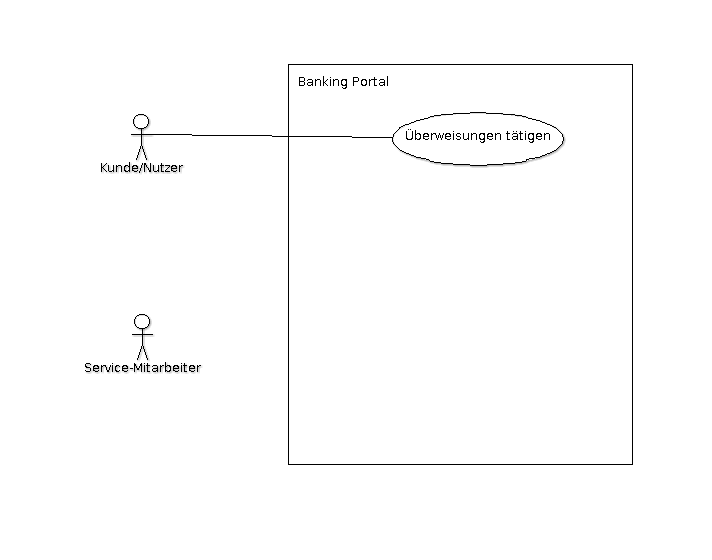
\includegraphics[width=0.95\linewidth]{Anwendungsfalldiagramm2}
\subsection*{Aufgabe 3}
\subsubsection*{a) Use Case ``Funktionalität einer Überweisung''}
\begin{tabular}{|p{0.37\linewidth}|p{0.57\linewidth}|}
\hline
\textbf{Use Case Abschnitt} & \textbf{Zweck} \\
\hline
Use Case Name & Tätigen einer Überweisung\\
\hline
Scope & Banking Portal \-- Unterpunkt Überweisung \\
\hline
Level & User Ziel\\
\hline
Primary Actor & Kunde\\
\hline
Stakeholders and Interests & Kunde \-- will Überweisungen tätigen, Bank \-- will vollständige Angaben zur Überweisung\\
\hline
Preconditions & Der Kunde hat sich authentifiziert und einen Überweisungstyp gewählt\\
\hline
Minimal guarantees & Es ist dem Kunden jederzeit klar, ob er eine Überweisung tätigen kann und wenn er es versucht, ab wann die Überweisung tatsächlich durchgeführt wird\\
\hline
Success Guarantee & Überweist der Kunde Geld, wird diese Transaktion den EIngaben entsprechend durchgeführt, auf allen beteiligten Konten vermerkt und mit einem Log-Eintrag vermerkt.\\
\hline
Main Success Scenario & 1. Der Kunde wählt im Web-Interface die Option, eine Überweisung aufzugeben \newline 2. Der Kunde gibt das Ziel der Überweisung in Form einer IBAN oder einer Kontonummer/Bankleitzahl-Kombination an. \newline 3. Der Kunde gibt den Geldbetrag an \newline 4. Der Kunde gibt einen Verwendungszweck bzw. eine Kundenreferenznummer an \newline 5. Der Kunde wählt exklusiv, ob die Überweisung sofort, zu einem bestimmten Termin oder regelmäßig erfolgen soll \newline 6. Der Kunde sendet das Formular ab \newline 7. Das System validiert die Eingaben, gibt dem Kunden ggf. Gelegenheit zur Korrektur und leitet bei korrekten Eingaben zur Zusammenfassungsseite weiter \newline 8. Das System gibt dem Kunden auf der Zusammenfassungsseite Auskunft über seine Angaben und fragt \-- abhängig vom gewählten Verfahren \-- die TAN ab bis die Eingabe entweder korrekt ist oder der Kunde die Überweisung abbricht \newline 9. Wurde die richtige TAN eingegeben gibt das System die Überweisung in Auftrag, bestätigt dem Kunden die Überweisung und bietet an, eine weitere Überweisung in Auftrag zu geben oder zum Hauptmenü zurück zu kehren\\
\hline
Extensions & Der Kunde kann Empfänger in einer Liste speichern und bei erneuten Überweisungen schnell auswählen (steht nicht im Text, aber sonst ist uns keine Erweiterung eingefallen) \\
\hline
Special Requirements & Der Kunde hat je nach gewähltem Verfahren die Möglichkeit die richtige TAN einzugeben \\
\hline
Technology and Data Variation List & Ggf. könnte es in Zukunft eine App geben, mit der man Überweisungen tätigen kann (steht nicht im Text) \\
\hline
Frequency of Occurrence & Täglich sehr häufig \\
\hline
Miscellaneous & \\
\hline
\hline
\end{tabular}

\subsubsection*{b) Use Case ``Neue TAN-Liste Versenden''}
\begin{tabular}{|p{0.37\linewidth}|p{0.57\linewidth}|}
\hline
\textbf{Use Case Abschnitt} & \textbf{Zweck} \\
\hline
Use Case Name & Versenden einer neuen TAN-Liste\\
\hline
Scope & Das zu entwickelnde System\\
\hline
Level & Funktion des Systems\\
\hline
Primary Actor & Das System\\
\hline
Stakeholders and Interests & \-- Der Nutzer will möglichst schnell eine neue TAN-Liste \newline \-- Die Bank will den Nutzer in einem sicheren Verfahren zuverlässig und schnell mit einer neuen TAN-Liste versorgen\\
\hline
Preconditions & Der Nutzer hat die TAN-Liste als Verfahren gewählt und entweder selbst das Versenden einer neuen Liste veranlasst oder eine TAN genutzt, dass nur noch maximal 10 TANs auf der Liste übrig sind \\
\hline
Minimal guarantees & Es wird nur in diesen begründeten Fällen eine TAN-Liste versandt\\
\hline
Success Guarantee & Der Nutzer erhält eine neue TAN-Liste\\
\hline
Main Success Scenario & 1. Der Nutzer veranlasst selbst mit einer TAN das Versenden einer neuen TAN-Liste oder er hat maximal 10 übrige TANs sodass das Versenden automatisch veranlasst wird. \newline 2. Hat er selbst das Versenden veranlasst wird, die alte Liste sofort gesperrt, sobald die neue Liste beantragt wurde 3. Der Kunde erhält die neue TAN-Liste 4. Wurde das Versenden automatisch veranlasst, werden mit der ersten Nutzung einer neuen TAN alle alten, noch gültigen TANs gesperrt. \\
\hline
Extensions & Der Kunde kann sehen wie viele gültige TANs er noch besitzt. (Steht nicht im Text)\\
\hline
Special Requirements & Das Versenden klappt möglichst schnell und transparent für den Kunden\\
\hline
Technology and Data Variation List & Keine \\
\hline
Frequency of Occurrence & Das Versenden neuer TAN-Listen gehört zum täglichen Geschäft \\
\hline
Miscellaneous & \\
\hline
\hline
\end{tabular}
\end{document}
